\subsection{Alastria ID Specification}
In this section we are going to see the different objects defined by Alastria for the model.
\subsubsection{DIDs}
As we have seen previously, the \acrfull{did}s are a type of identifier that allows the verification of decentralized identities. It should be noted that all entities, regardless of their role, have a \acrshort{did} that identifies them. At Alastria, the W3C standard is followed with a few minor differences.
\begin{itemize}
    \item It will include the type of network in which the \acrshort{did} has been registered.
    \item It will also include the blockchain network and the network ID where the \acrshort{did} is registered.
\end{itemize}

Alastria \acrshort{did}s have the following format (listing \ref{lst:did_format}):
\lstinputlisting[label={lst:did_format}, caption=\acrshort{did} format]{examples/codeSnippets/did_format.txt}
Where:
\begin{itemize}
    \item \textbf{"ala"}: specifies that this is a \acrshort{did} for Alastria.
    \item \textbf{"network"}: specifies the technology used on that network.
    \item \textbf{"net-id"}: defines the specific Alastria blockchain network instance.
\end{itemize}
Possible examples of \acrshort{did}s are (listing \ref{lst:did_ex}):
\lstinputlisting[label={lst:did_ex}, caption=Examples of \acrshort{did}s]{examples/codeSnippets/did_examples.txt}

\subsubsection{Artifacts}
Alastria Artifacts are currently coded as \acrshort{jwt} objects, so they follow the \acrshort{jwt} specification previously explained.

The header has the following arguments:
\begin{itemize}
    \item \textbf{"alg"}: the hashing algorithm.
    \item \textbf{"typ"}: type of the object. It will always be \textit{"\acrshort{jwt}"}.
    \item \textbf{"kid"}: it is an optional attribute. It is the identifier of the public key of the issuer of the \acrshort{jwt}. It may not be the key the \acrshort{jwt} was signed with.
    \item \textbf{"jwk"}: it is an optional attribute. It is the public key used to sign the \acrshort{jwt}.
\end{itemize}
For the payload, there are some common attributes, but they are all optional.
\begin{itemize}
    \item \textbf{"jti"}: \acrshort{jwt} unique identifier.
    \item \textbf{"iat"}: "issued at". Token issue date.
    \item \textbf{"nbf"}: "not before". Token activation date.
    \item \textbf{"exp"}: token expiration date.
\end{itemize}
The different artifacts, their specific payloads and their utility will be explained below.

\paragraph{Alastria Token (AT)}
It is a token that allows an issuer to identify a subject that does not have a \acrshort{did} or does not know it yet. This object is used by other objects, such as \acrfull{aic} and \acrfull{as}.

This object has the following payload:
\begin{itemize}
    \item \textbf{"gwu"}: Gateway \acrshort{url}.
    \item \textbf{"cbu"}: Callback \acrshort{url}.
    \item \textbf{"iss"}: \acrshort{did} of the token issuer.
    \item \textbf{"ani"}: Alastria network identifier.
\end{itemize}
In the next listing (listing \ref{lst:at_ex}) we can see an example of a decoded \acrlong{at}.
\lstinputlisting[language=json,label={lst:at_ex}, caption=Decoded \acrlong{at} example]{examples/codeSnippets/at.json}

\paragraph{Alastria Session (AS)}
It is a token that is used to authenticate users when they want to do an on-boarding with Alastria ID.

This object has the following payload:
\begin{itemize}
    \item \textbf{"@context"}: an array of \acrshort{url}s with the allowed specification.
    \item \textbf{"iss"}: \acrshort{did} of the token issuer. It is usually a subject.
    \item \textbf{"alastriaToken"}: the signed \acrlong{at} issued by the entity.
    \item \textbf{"pku"}: public key of the token issuer.
\end{itemize}
In the next listing (listing \ref{lst:as_ex}) we can see an example of a decoded \acrlong{as}.
\lstinputlisting[language=json,label={lst:as_ex}, caption=Decoded \acrlong{as} example]{examples/codeSnippets/as.json}

\paragraph{Alastria Identity Creation (AIC)}
It is a token used only in identity creation (\acrshort{did}).

This object has the following payload:
\begin{itemize}
    \item \textbf{"createAlastriaTX"}: it is the signed transaction of the \textit{"createAlastriaIdentity"}\footnote{\url{https://github.com/alastria/alastria-identity/blob/master/contracts/identityManager/AlastriaIdentityManager.sol\#L59}} function from the \textit{AlastriaIdentityManager} smart contract, signed by the subject.
    \item \textbf{"alastriaToken"}: verified \acrlong{at}, signed by the issuer entity.
    \item \textbf{"publicKey"}: subject's Public Key.
\end{itemize}
In the next listing (listing \ref{lst:aic_ex}) we can see an example of a decoded \acrlong{aic}.
\lstinputlisting[language=json,label={lst:aic_ex}, caption=Decoded \acrlong{aic} example]{examples/codeSnippets/aic.json}

\paragraph{Credential}
A credential is a piece of information said and verified by an Issuer on a Subject. That is, it is created by an Issuer and received by a Subject. It should be noted that in Alastria when talking about credentials, they are talking about verifiable credentials (explained previously) that are the only ones that are useful in the context of \acrlong{ssi}.

This object has the following payload:
\begin{itemize}
    \item \textbf{"sub"}: the subject. It is to whom the credential is addressed.
    \item \textbf{"iss"}: the issuer (normally with the issuer role) of the credential.
    \item \textbf{"vc"}: "VerifiableCredential". It is a \acrshort{json} that contains the credential data and some metadata. The content is:
          \begin{itemize}
              \item \textbf{"@context"}: an array of \acrshort{url}s with the allowed specification.
              \item \textbf{"type"}: the type of the object. At a minimum it must have \textit{"VerifiableCredential"} and \textit{"AlastriaVerifiableCredential"}. additionally it can have more.
              \item \textbf{"credentialSubject"}: a \acrshort{json} with the credential data itself. This attribute is also a \acrshort{json} with an optional attribute \textbf{"levelOfAssurance"}, which is the minimum \acrlong{loa} that the credential must meet (it will be explained later); and the rest of the fields correspond to the standard claim names in \acrshort{jwt}.
          \end{itemize}
\end{itemize}
In the following listing (listing \ref{lst:cred_ex}) we can see an example of a Credential issued to certify the issuance of a title for a person.
\lstinputlisting[language=json,label={lst:cred_ex}, caption=Decoded Credential example]{examples/codeSnippets/credential.json}

\paragraph{Presentation Request (PR)}
A Presentation Request, normally known as \textit{"PR"} is a token to request a set of credentials, it is requested normally by a Service Provider. It means that is issued by a Service Provider and received by a Subject, in order to provide a specific service to the subject.

This object has the following payload:
\begin{itemize}
    \item \textbf{"cbu"}: the callback \acrshort{url}.
    \item \textbf{"pr"}: \textit{"Presentation Request"}. It is a \acrshort{json} that contains the presentation request data and its metadata. It's content is:
          \begin{itemize}
              \item \textbf{"type"}: the type of object. At a minimum it must have \textit{"VerifiablePresentation"} and \textit{"AlastriaVerifiablePresentation"}. Additionally it can have more.
              \item \textbf{"@context"}: an array of \acrshort{url}s with the allowed specification.
              \item \textbf{"procUrl"}: \acrshort{url} of the external document that explains the use that will be given to the credentials.
              \item \textbf{"procHash"}: hash of the external document that explains the use that will be given to the credentials.
              \item \textbf{"data"}: \acrshort{json} array containing the presentation request data. Each \acrshort{json} is only for one credential, and has the following format:
                    \begin{itemize}
                        \item \textbf{"@context"}: allowed credential specification.
                        \item \textbf{"field\_name"}: Credential requested.
                        \item "\textbf{required"}: a boolean that indicates whether it is a mandatory field or not.
                        \item \textbf{"levelOfAssurance"}: it is the minimum \acrfull{loa} that the credential must meet. This will be explained later
                    \end{itemize}
          \end{itemize}
\end{itemize}
In the following listing (listing \ref{lst:pr_ex}) we can see an example of a Presentation Request issued to request a person's data for a COVID test.
\lstinputlisting[language=json,label={lst:pr_ex}, caption=Decoded Presentation Request example]{examples/codeSnippets/pr.json}

\paragraph{Presentation}
A Presentation is the response to a Presentation Request. It is emitted by a subject for a Service Provider, it means that the object is signed by the subject. It consists of the collection of one or more credentials issued by one or more Issuers.

This object has the following payload:
\begin{itemize}
    \item \textbf{"iss"}: it is the Issuer of the Presentation. In most cases, it is a Subject.
    \item \textbf{"aud"}: "Audience". He is the recipient of the presentation. It is normally a Service Provider.
    \item \textbf{"vp"}: "Verifiable Presentation". It is a \acrshort{json} that contains the presentation data and its metadata. It consists in:
          \begin{itemize}
              \item \textbf{"type"}: the type of the object. At a minimum it must have \textit{"VerifiablePresentation"} and \textit{"AlastriaVerifiablePresentation"}. Additionally it can have more.
              \item \textbf{"@context"}: allowed presentation specification.
              \item \textbf{"procUrl"}: \acrshort{url} of the external document that explains the use that will be given to the credentials.
              \item \textbf{"procHash"}: hash of the external document that explains the use that will be given to the credentials.
              \item \textbf{"verifiableCredential"}: an array of signed Credentials (signed \acrshort{jwt}s).
          \end{itemize}
\end{itemize}
In the next listing (listing \ref{lst:pres_ex}) we can see an example of a decoded Presentation.\\
\lstinputlisting[language=json,label={lst:pres_ex}, caption=Decoded Presentation example]{examples/codeSnippets/presentation.json}

At the moment no more objects have been defined, but if it is necessary to explain some peculiarities of the model with respect to the previous objects.

\paragraph{Level Of Assurance (LOA)}
The Credentials and Presentation Requests can have an attribute called \textit{"levelOfAssurance}, which is the \acrfull{loa}. It corresponds to the \acrshort{eidas} assurance levels\footnote{\url{https://www.eid.as/\#article8}} (\textit{"Low"}, \textit{"Substantial"}, \textit{"High"}), plus an additional lower level \textit{"Self"} for self-asserted data. \\

The actual level depends on the entity making the Credential and the process used by the entity to verify the attribute. If the field does not exist in the Credential, the verifier will have to use the knowledge that it has about the issuing entity in order to assess the risks associating with accepting that credential.

\paragraph{Private Sharing Multi Hashes (PSMHash)}
Mostly known as \acrshort{psmh} is a hash operation where the \acrshort{did} and the Credential or Presentation are concatenated. This means, that each credential/presentation has two ways of being identified. By the \acrshort{psmh} of the Subject or by the \acrshort{psmh} of the entity.

The figure \ref{fig:psmh} shows an schema for the \acrshort{psmh} for the Credentials and the Presentations.
\begin{figure}[h]
    \centering
    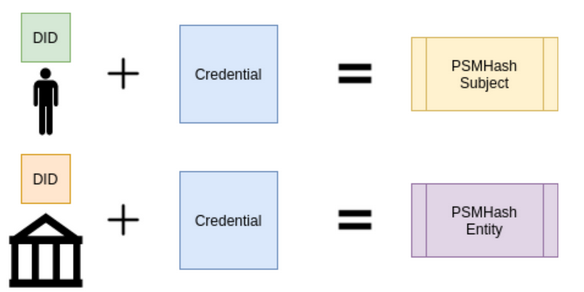
\includegraphics[width=.5\textwidth]{psmhash-credential.png}\hfill
    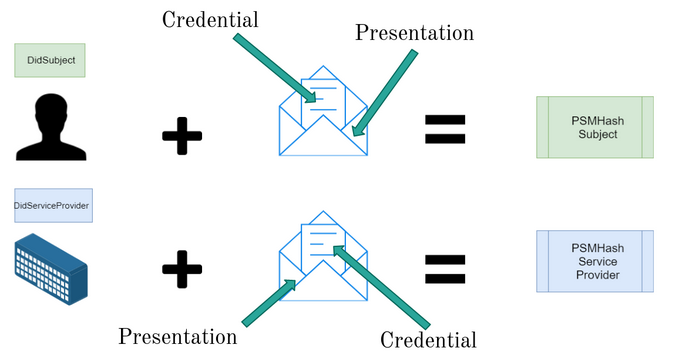
\includegraphics[width=.5\textwidth]{psmhash-presentation.png}
    \caption{\acrshort{psmh} schema for Credentials and Presentations}
    \label{fig:psmh}
\end{figure}

With the \acrshort{psmh} is guaranteed that only the parties involved can "understand" those hashes when they are issued on the blockchain, since it is not the Credential or Presentation itself (the \acrshort{jwt}s) that is transacted on the blockchain, but their \acrshort{psmh}es.

\paragraph{Status of Credentials and Presentations}
As explained in the previous paragraph, both the Credentials and the Presentations have two ways of being identified, therefore, each of the \acrshort{psmh} has an associated status in the blockchain.

For \textbf{Credentials}, the possible statuses are:
\begin{itemize}
    \item \textbf{"0"} or \textbf{"Valid"}: status the Credential has when issued by an Issuer.
    \item \textbf{"1"} or \textbf{"AskIssuer"}: this status implies that the Issuer of the Credential wants to be asked what the real status of that Credential is.
    \item \textbf{"2"} or \textbf{"Revoked}: status of the Credential when the issuer revokes it for any reason.
    \item \textbf{"3"} or \textbf{"DeletedBySubject"}: status when the Subject has removed the Credential.
\end{itemize}

Similarly, \textbf{Presentations} have the following statuses:
\begin{itemize}
    \item \textbf{"0"} or \textbf{"Valid"}: status the Presentation has when issued by a Subject.
    \item \textbf{"1"} or \textbf{"Received"}: status that the Presentation gets when it is received by a Service Provider.
    \item \textbf{"2"} or \textbf{"AskDeletion"}: status that the Subject puts when he wants the Presentation to be eliminated and therefore the Credentials that it contains are not used.
    \item \textbf{"3"} or \textbf{"DeletionConfirmation"}: status that the Service Provider puts in the Presentation when confirming the deletion requested by the Subject previously.
\end{itemize}

